%global style
\documentclass[a4paper]{book}
\usepackage{CJK}

%predined style
%--------------------------------------------
\usepackage{graphicx}

%--------------------------------------------
\usepackage{color}

%--------------------------------------------
\usepackage{minted}
%new command can be used like this:
%
% \begin{ccode}
% ...
% \end{ccode}
\newminted{c}{linenos,fontsize=\normalsize}
\newminted{v}{linenos,fontsize=\normalsize}
\newminted{sh}{linenos,fontsize=\normalsize}
\newminted{python}{linenos,fontsize=\normalsize}
\newminted{text}{linenos,fontsize=\normalsize}
\newminted{diff}{linenos,fontsize=\normalsize}

%linenos font style
\renewcommand{\theFancyVerbLine} {
    \small\textcolor[rgb]{0.5,0.5,1.0}{
    \arabic{FancyVerbLine}}}

%--------------------------------------------
\usepackage{fancyhdr}
\pagestyle{fancy}

\fancyhead{}
\fancyhead[RE, LO]{\leftmark}
\fancyhead[LE, RO]{\thepage}
\renewcommand{\headrulewidth}{0.4pt} 

\fancyfoot{}
%\fancyfoot[LE, RO]{\bfseries Using PicoBlaze}
\fancyfoot[LE, RO]{\color{gray} Creative Commons Attribution-NonCommercial 3.0}
%\fancyfoot[CE, CO]{}
\fancyfoot[RE, RO]{\color{gray} \LaTeXe}
%\renewcommand{\footrulewidth}{0.4pt}

%--------------------------------------------
%\usepackage{listings}
%\lstset{numbers=left,
%    numberstyle=\small\color[rgb]{0.5,0.5,1.0},
%    frame=none,
%    flexiblecolumns=false,
%    language=Python,
%    basicstyle=\ttfamily\normalsize,
%    breaklines=true,
%    extendedchars=true,
%    escapechar=\\,
%    texcl=true,
%    showstringspaces=none,
%    keywordstyle=\bfseries,
%    tabsize=4}

%--------------------------------------------
\usepackage{indentfirst}
\usepackage[colorlinks=true, pdfstartview=FixW, CJKbookmarks=true]{hyperref}



%--------------------------------------------
\begin{document} \begin{CJK*}{UTF8}{song} \large
%begin of document

\title{Using PicoBlaze}
\author{buaa.byl@gmail.com}
\date{\today}
\maketitle
\tableofcontents

%*******************************************************************************
\chapter{Introduction}
转眼自己工作四年了,在这四年里做过的东西太杂,涉及到的技术太多,
如果不整理一下过几年就会渐渐的忘记,那么这四年就只是经历而不能成为经验。
我在学校里学的是芯片设计,学的主要是电子系的课程,
没有系统的学过计算机系的课程。毕业后主要做的是嵌入式系统开发,
先分析uIP和lwip的实现,再以此为基础实现了一个专用的协议栈
(属于令牌网,要求实时通信)。而后转作FPGA的设计和开发、
顺带编写上位机驱动,编写过各种脚本。

曾经有个Palm TT5,上面有个圣经软件BiblePlus,
我发现电子版的圣经数据有些错误,于是自己抽空分析Bibleplus的数据格式,
并用c写了一个解析程序,可以解码圣经,修正,然后再编码。可惜后来我的Palm坏了。
于是把代码共享到Google Code,居然有人发邮件联系我提交Bug!
说实在真没想到自己的代码居然有人觉得有用。
但悲剧的是自己看不懂自己的代码了:(

后来自己把CF卡DIY为固态硬盘(那个时候还没有廉价的SSD),
于是做了EWF、FBWF的界面,也有人觉得有用,发邮件给我提需求。
经过这些备受鼓励,于是就想着能不能写点东西。

现在应该就是一个契机,自己想弄一个以太网通信控制器,
实现轻量级的TCPIP协议栈。因为目的是梳理知识,而不是做产品,
所以没必要考虑用ARM来做。

我的想法是先阅读PicoBlaze软核,再从底层往上走。
梳理出最简单的CPU设计方法,可以总结出一些基本的原则,
可以方便的编写符合自己需求的CPU,然后是添加调试接口,
工具链移植,通信接口。最后用多个CPU核实现一个“硬件”TCPIP协议栈。
\\

我从PicoBlaze的使用开始写起,分析它的指令集,如何使用。
如何写一个简单的汇编处理器,自己比较熟悉Python,
所以就用简单的Python脚本来做。

然后开始分析用原语写的PicoBlaze,并把它改写为RTL。
顺带写个汇编预处理器,可以支持一些简单的宏。
再给PicoBlaze添加Jtag调试接口,这个之前没做过,
所以会比较慢,还不知道会弄多久。
移植GCC到新的平台是一件很庞大的工程,
如果要自己写微处理器这一步没法省略的,
所以先从分析别人的工作开始,学习移植步骤,
然后再尝试自己移植。
SPI和UART是常见的两种外设接口,所以在这里一并实现。
后续会计划在上面的基础上写协议栈,可能还要写一个简单的SDRAM控制器。
毕竟网络的数据量是比较大的,光用Block RAM可能不够。
\\

本书打算在今年写完,用\LaTeXe来排版,中英文交替着写,也练习英文写作。
这就当复习如何写论文了:)

\clearpage
\section{KCPSM3}
$PicoBlaze^{\textregistered{}}$是$Xilinx^{\textregistered{}}$针对低端应用开发的8位处理器,
开放源代码。

PicoBlaze另一个名称KCPSM,是Constant(K) Coded Programmable State Machine的简称,
也即常量编码状态机。由Ken Chapman开发,所以也有人这么理解Ken Chapman's PSM。

本文分析的主要是Spartan3系列的版本,即KCPSM3,
典型的KCPSM3占用96个Slices,等价于低端XC3S200器件5\%的资源。

PicoBlaze是8位处理器,使用18位指令集,每个指令执行时间为2个周期。 
KCPSM3直接用xilinx原语编写,只有汇编器。这样就导致在使用中有些问题,
其一汇编维护起来太麻烦,其次想添加新的指令很难。

而PicoBlaze只有一份很旧的设计说明,还是针对停产的VertixII器件的。
这篇文章是“Creating Embedded Microcontrollers (Programmable State Machines)”,
很值得一读,不过还是旧了一点。
PicoBlaze缺少一个完整的设计文档,当然也没找到KCPSM3的设计说明。
所以想要修改它其实非常不容易,我准备阅读它的源码,归纳设计的方法。
虽然已经有现成的PacoBlaze\footnote{PacoBlaze:一个基于PicoBlaze的开源实现},
但想要方便以后的使用,还是自己阅读源码,并改写为Verilog。
再次说一句我的目的是梳理知识:)

\clearpage
\section{Application of PicoBlaze}
\begin{enumerate}
\item LED flasher.
\item PWM control and even generation.
\item Switch monitor.
\item UART interface and simple command/status terminal.
\item LCD character module display interface and control.
\item SPI master
\item I2C master.
\item Calculator.
\item Audio DSP processor.
\item DTMF tone telephone dialer including sine wave generation.
\item System monitoring.
\item Motor control.
\item Rotary encoder interface.
\item Calculator for frequency synthesizer.
\item Calculator for filter coefficient generation.
\item Emulation of a different micro controller.
\item PID control.
\item Mouse/Keyboard interface.
\item Keypad scanner.
\item Power supply monitoring and control.
\item Servo control.
\item Built-in test equipment.
\item Configuration management.
\item Design Authentication Processor.
\item Implementing peripherals for MicroBlaze or PPC.
\item Interrupt controller for MicroBlaze or PPC.
\end{enumerate}

\section{Code style}
\textbf{c code style:}
\begin{ccode}
int adder(int a, int b)
{
    return a + b;
}
\end{ccode}

\textbf{verilog code style:}
\begin{vcode}
module adder(input a, 
        input b,
        output c);

assign c = a + b;

endmodule
\end{vcode}



\part{Using KCPSM3}
\chapter{How to store code}
\chapter{What assembler generated}
\chapter{Instruction set}
\chapter{Assembler in python}

\part{Reading KCPSM3}
\chapter{Architecture}
\chapter{Interrupt}

阅读代码需要一个开始的地方,因为PicoBlaze定位是可编程状态机,
那么就从外部中断开始阅读,中断包含同步、使能、上下文切换。

\section{int\_capture\_flop}
我们先从外部中断引脚开始看,看看经过哪些逻辑。以下是picoblaze的顶层接口:

\begin{vcode}
module kcpsm3(
        address,
        instruction,
        port_id,
        write_strobe,
        out_port,
        read_strobe,
        in_port,
        interrupt,
        interrupt_ack,
        reset,
        clk) ;
 
output  [9:0]   address ;
input   [17:0]  instruction ;
output  [7:0]   port_id ;
output          write_strobe, read_strobe, interrupt_ack ;
output  [7:0]   out_port ;
input   [7:0]   in_port ;
input           interrupt, reset, clk ;
\end{vcode}


\newpage
可以从字义上理解interrupt为外部中断的入口,而interrupt\_ack为中断确认信号,interrupt首先连入int\_capture\_flop逻辑:

\begin{vcode}
// Interrupt capture
FDR int_capture_flop (
    .D(interrupt),
    .Q(clean_int),
    .R(internal_reset),
    .C(clk));
\end{vcode}

在Synplify的Technology View可以看到如下的图\\
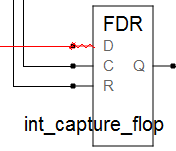
\includegraphics{int_capture_flop.png}

这个FDR是“同步复位D触发器”原语。FDR是比较好理解的,D是输入,Q是输出,R是复位,C是时钟。\\
在\verb|C:\Xilinx\12.4\ISE_DS\ISE\verilog\xeclib\unisims|下是官方给出的仿真代码。
在后面还会涉及到LUT(查找表),所以在这里先介绍一下。

\textbf{FDR}
\begin{vcode}
module FDR (Q, C, D, R);
    parameter INIT = 1'b0;
    output Q;
    reg    Q;
    input  C, D, R;
    always @(posedge C)
        if (R)
        Q <= 0;
        else
        Q <= D;
endmodule
\end{vcode}

\textbf{LUT4}
\begin{vcode}
module LUT4 (O, I0, I1, I2, I3);
    parameter INIT = 16'h0000;
    input I0, I1, I2, I3;
    output O;
    wire out0, out1, out2, out3, out;
    assign O = INIT[{I3,I2,I1,I0}];
endmodule
\end{vcode}

FDR就是一个触发器,LUT4是一个16bit的ROM结构,O是输出,I3、I2、I1、I0是地址线。

因为原语不太直观,所以在这里把\verb|int_capture_flop|改写为rtl描述。

\begin{vcode}
always@(posedge clk)
begin
    if (internal_reset)
        clean_int <= 1'b0;
    else
        clean_int <= interrupt;
end
\end{vcode}

这个逻辑同步外部的中断信号。interrupt是外部中断信号,\verb|clean_int|是同步后的中断信号。 \verb|internal_reset|是PicoBlaze内部复位信号,当处理器复位的时候,\verb|internal_reset|会持续一段时间。

用原语来写有个好处就是综合的结果基本上就是你想要的电路,
但代价就是不容易维护,也不利于别人阅读。

\clearpage
\section{Karnaugh Graphic}
用原语来写逻辑就需要用上卡诺图,
而阅读用原语写的组合逻辑代码更需要卡诺图!
因为LUT的值是一个16位的数字,很不直观,于是想到自己写个脚本
把16位的值转为一个平面的图。

\textbf{karnaugh.py}
\begin{pythoncode}
#!/bin/python
import sys

def itob(a, bitnum=16):
    bits = []
    for i in range(0, bitnum):
        if (a & (1 << (bitnum - 1 - i))) != 0:
            bits.append('1')
        else:
            bits.append('0')
    return bits

def printv(bits):
    #dec format index
    sys.stdout.write('bitno: ')
    for i in range(15, -1, -1):
        sys.stdout.write('%4d' % i)
        if (i % 4) == 0:
            sys.stdout.write(' | ')
        else:
            sys.stdout.write(' ')
    sys.stdout.write('\n')

    #binary format index
    sys.stdout.write('bitno: ')
    for i in range(15, -1, -1):
        sys.stdout.write(''.join(itob(i, bitnum=4)))
        if (i % 4) == 0:
            sys.stdout.write(' | ')
        else:
            sys.stdout.write(' ')
    sys.stdout.write('\n')

    #value
    sys.stdout.write('value: ')
    bitno = 15
    for bit in bits:
        sys.stdout.write('%4s' % bit)
        if (bitno % 4) == 0:
            sys.stdout.write(' | ')
        else:
            sys.stdout.write(' ')
        bitno -= 1
    sys.stdout.write('\n')
    sys.stdout.write('\n')

    #karnaugh map
    print('kano-graphic:')
    sys.stdout.write('||= bit(3210) =|' + \
            '|=  xx11 =||=  xx10 =||=  xx00 =||=  xx01 =||\n')
    
    sys.stdout.write('||         11xx||%7s  ||%7s  ||%7s  ||%7s  ||\n' % (
        bits[0*4 + 0], bits[0*4 + 1], bits[0*4 + 3], bits[0*4 + 2]))
    
    sys.stdout.write('||         10xx||%7s  ||%7s  ||%7s  ||%7s  ||\n' % (
        bits[1*4 + 0], bits[1*4 + 1], bits[1*4 + 3], bits[1*4 + 2]))
    
    sys.stdout.write('||         00xx||%7s  ||%7s  ||%7s  ||%7s  ||\n' % (
        bits[3*4 + 0], bits[3*4 + 1], bits[3*4 + 3], bits[3*4 + 2]))
    
    sys.stdout.write('||         01xx||%7s  ||%7s  ||%7s  ||%7s  ||\n' % (
        bits[2*4 + 0], bits[2*4 + 1], bits[2*4 + 3], bits[2*4 + 2]))
    sys.stdout.write('\n')

def printlut4(a):
    bits = itob(a)
    print('original: 0x%04X' % a)
    print
    printv(bits)

if __name__ == '__main__':
    if len(sys.argv) == 1:
        print 'need hex digit!'
    else:
        printlut4(int(sys.argv[1], 16))

\end{pythoncode}



对于0x1010,转换的结果如下:
\begin{textcode}
kano-graphic:
||= bit(3210) =||=  xx11 =||=  xx10 =||=  xx00 =||=  xx01 =||
||         11xx||      0  ||      0  ||      1  ||      0  ||
||         10xx||      0  ||      0  ||      0  ||      0  ||
||         00xx||      0  ||      0  ||      0  ||      0  ||
||         01xx||      0  ||      0  ||      1  ||      0  ||
\end{textcode}
这样就很容易弄清楚逻辑关系了:)


\chapter{Interrupt Logic}
\chapter{Flow Control}
\chapter{PC and Registers}
\chapter{Store Memory}
\chapter{Call Stack}
\chapter{ALU and Multiplexer}
\chapter{Input and output}
\chapter{Rewrite KCPSM3 in verilog}
\chapter{Assembler preprocessor in python}

\part{JTAG}
\chapter{Missing debug}
\chapter{What is jtag}
\chapter{Jtag slave in verilog}
\chapter{Jtag master in c}
\chapter{A stm32-based jtag master}
\chapter{A kcpsm3-base jtag master}
\chapter{Add breakpoint controler}
\chapter{Add boundary scan to kcpsm3}
\chapter{Reuse lattice mico8 gcc}

\part{Port GCC}
\chapter{What lm8-gcc do}
Xilinx有8位的PicoBlaze处理器,Lattice也有一个8位的处理器Mico8。
以下是PicoBlaze的系统框架图\footnote{图片来自PicoBlaze Manual.pdf,Page8} \\
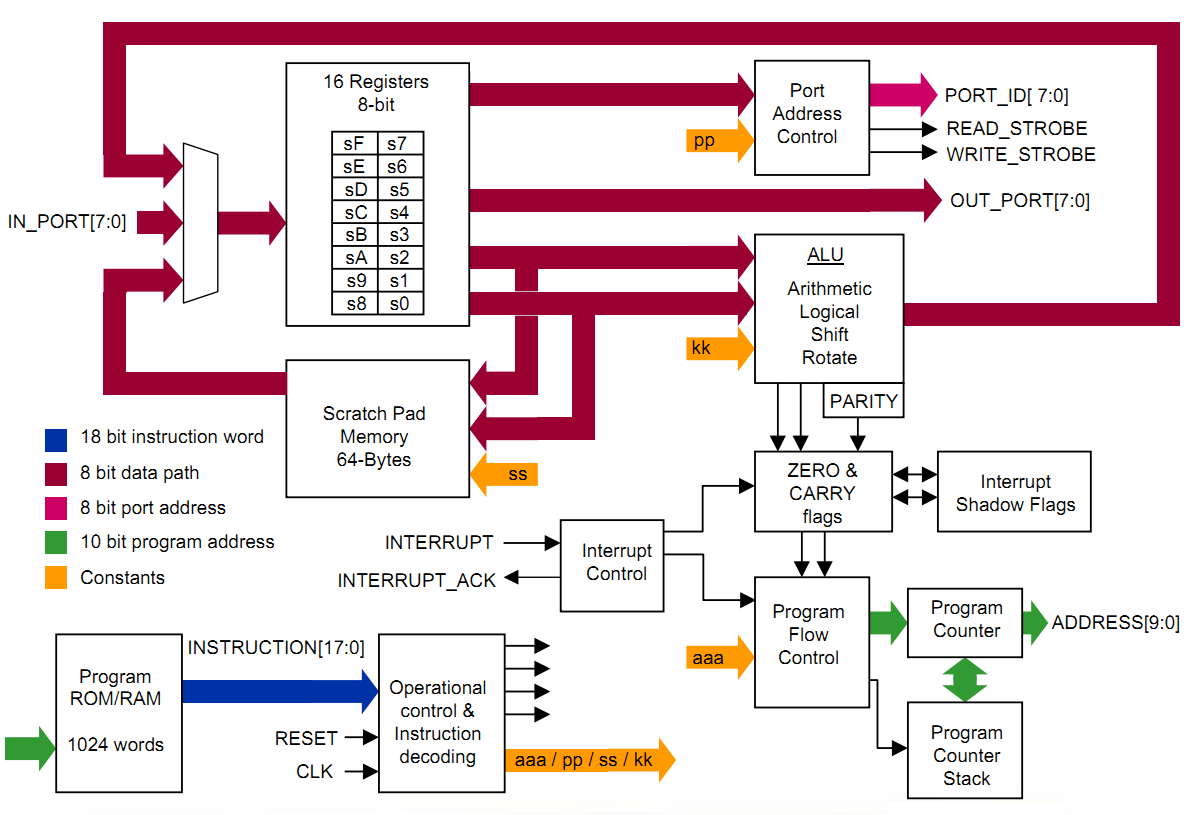
\includegraphics[width=\textwidth]{pb8arch}

这个是Mico8的系统框架图\footnote{图片来自rd1026.pdf,Page1} \\
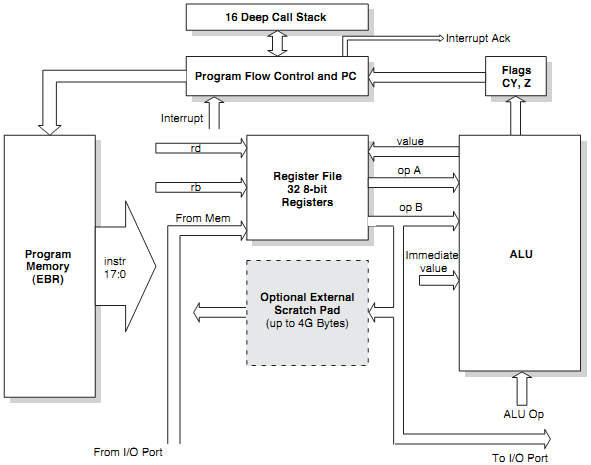
\includegraphics[width=\textwidth]{lm8arch}

仔细看系统框图,发觉Mico8和PicoBlaze的设计很相似。
更让人惊喜的是Lattice已经移植了Mico8版本的GCC,这样意味着很有可能把这个
GCC修改一下支持PicoBlaze!
也可以学习移植GCC,毕竟gcc的x86、arm、sparc都不简单。

\clearpage
\section{Compare}
既然要想弄明白Lattice是怎么移植GCC的,那么最好的办法就是
找出lm8-gcc和原始的gcc之间的差异,然后对比差异来学习。

这么一来第一件事就是找到两份源代码,一个是lm8-gcc,另一个是原始的gcc。
在Lattice找到了LatticeMico8\_Tools\_v3\_15的链接,
下载回来是 gcc-lm8-2010-09-28.tar.bz2,这个就是移植Mico8的gcc。
解压后可以知道这个gcc-lm8是以GCC 4.4.3为基础改出来的。
那么我们再到GCC的ftp把 gcc-4.4.3.tar.bz2 下载回来。

我把lm8-gcc的源码解压为gcc-4.4.3-lm8,把原始的gcc解压为gcc-4.4.3-org。
需要对比差异,最简单的就是使用diff工具,在linux下这个工具常用来生成patch文件。

至于diff怎么用,直接输入以下命令:
\begin{shcode}
#/bin/sh
diff --help
\end{shcode}

输出如下:
\begin{textcode}
Usage: diff [OPTION]... FILE1 FILE2

  -i  --ignore-case  Consider upper- and lower-case to be the same.
  -w  --ignore-all-space  Ignore all white space.
  -b  --ignore-space-change  Ignore changes in the amount of white space.
  -B  --ignore-blank-lines  Ignore changes whose lines are all blank.
  -I RE  --ignore-matching-lines=RE  Ignore changes whose lines all match RE.
  --binary  Read and write data in binary mode.
  -a  --text  Treat all files as text.

  -c  -C NUM  --context[=NUM]  Output NUM (default 2) lines of copied context.
  -u  -U NUM  --unified[=NUM]  Output NUM (default 2) lines of unified context.
    -NUM  Use NUM context lines.
    -L LABEL  --label LABEL  Use LABEL instead of file name.
    -p  --show-c-function  Show which C function each change is in.
    -F RE  --show-function-line=RE  Show the most recent line matching RE.
  -q  --brief  Output only whether files differ.
  -e  --ed  Output an ed script.
  -n  --rcs  Output an RCS format diff.
  -y  --side-by-side  Output in two columns.
    -w NUM  --width=NUM  Output at most NUM (default 130) characters per line.
    --left-column  Output only the left column of common lines.
    --suppress-common-lines  Do not output common lines.
  -DNAME  --ifdef=NAME  Output merged file to show `#ifdef NAME' diffs.
  --GTYPE-group-format=GFMT  Similar, but format GTYPE input groups with GFMT.
  --line-format=LFMT  Similar, but format all input lines with LFMT.
  --LTYPE-line-format=LFMT  Similar, but format LTYPE input lines with LFMT.
    LTYPE is `old', `new', or `unchanged'.  GTYPE is LTYPE or `changed'.
    GFMT may contain:
      %<  lines from FILE1
      %>  lines from FILE2
      %=  lines common to FILE1 and FILE2
      %[-][WIDTH][.[PREC]]{doxX}LETTER  printf-style spec for LETTER
        LETTERs are as follows for new group, lower case for old group:
          F  first line number
          L  last line number
          N  number of lines = L-F+1
          E  F-1
          M  L+1
    LFMT may contain:
      %L  contents of line
      %l  contents of line, excluding any trailing newline
      %[-][WIDTH][.[PREC]]{doxX}n  printf-style spec for input line number
    Either GFMT or LFMT may contain:
      %%  %
      %c'C'  the single character C
      %c'\OOO'  the character with octal code OOO

  -l  --paginate  Pass the output through `pr' to paginate it.
  -t  --expand-tabs  Expand tabs to spaces in output.
  -T  --initial-tab  Make tabs line up by prepending a tab.

  -r  --recursive  Recursively compare any subdirectories found.
  -N  --new-file  Treat absent files as empty.
  -P  --unidirectional-new-file  Treat absent first files as empty.
  -s  --report-identical-files  Report when two files are the same.
  -x PAT  --exclude=PAT  Exclude files that match PAT.
  -X FILE  --exclude-from=FILE  Exclude files that match any pattern in FILE.
  -S FILE  --starting-file=FILE  Start with FILE when comparing directories.

  --horizon-lines=NUM  Keep NUM lines of the common prefix and suffix.
  -d  --minimal  Try hard to find a smaller set of changes.
  -H  --speed-large-files  Assume large files and many scattered small changes.

  -v  --version  Output version info.
  --help  Output this help.

If FILE1 or FILE2 is `-', read standard input.
\end{textcode}

这个说明是很详细的,基本上不用再多说什么了。

我使用以下的命令对比。参数u是添加行号;N是如果文件是新增的,那么把源文件当成空的;r是递归调用。
(由于GCC源码太大,对比的时间很长,耐心等候吧)
\begin{shcode}
#/bin/sh
diff -uNr gcc-4.4.3-org gcc-4.4.3-lm8 > result.diff
\end{shcode}

得到差异结果有130Kb,不方便阅读,也不方便贴出来,所以自己写个简单的python脚本提取文件名。
这样就相当于有了一个索引,阅读和定位都方便很多。

\textbf{diffbrief.py}
\begin{pythoncode}
#!/bin/python
import sys, re

fin = open(sys.argv[1])
lines = fin.read()
fin.close()

regex_prefix = re.compile(r'^diff -uNr ')
regex_header = re.compile(r'^diff -uNr ([^ ]+) ([^ ]+)')
lineno = 1

for line in lines.split('\n'):
    if regex_prefix.match(line):
        res = regex_header.search(line)
        relative_path = res.groups()[0]
        relative_path = '/'.join(relative_path.split('\\')[1:])
        print '%04d: %s' % (lineno, relative_path)
    lineno += 1
\end{pythoncode}



输出的结果如下,其中左边的数字是每个被修改的文件在result.diff的行号,右边是被修改的文件的位置:
\begin{textcode}
0001: config.sub
0032: configure
0045: configure.ac
0058: gcc/config/lm8/constraints.md
0087: gcc/config/lm8/crt0.S
0177: gcc/config/lm8/libgcc.S
1878: gcc/config/lm8/lm8-protos.h
1951: gcc/config/lm8/lm8.c
3795: gcc/config/lm8/lm8.h
4427: gcc/config/lm8/lm8.md
5082: gcc/config/lm8/lm8.opt
5127: gcc/config/lm8/predicates.md
5192: gcc/config/lm8/t-lm8
5261: gcc/config/gcc
5284: libgcc/config/lm8/t-default
5291: libgcc/config.host
\end{textcode}
例如:需要找libgcc/config.host的修改,可以到result.diff的5291行。

\clearpage
\section{Summary}
对照源码的目录之后知道,gcc/config/lm8 和 libgcc/config/lm8 这两个目录是不存在的,
所以可以总结出对比的结果:
\begin{enumerate}
    \item 新文件
    \begin{itemize}
        \item gcc/config/lm8/constraints.md
        \item gcc/config/lm8/crt0.S
        \item gcc/config/lm8/libgcc.S
        \item gcc/config/lm8/lm8-protos.h
        \item gcc/config/lm8/lm8.c
        \item gcc/config/lm8/lm8.h
        \item gcc/config/lm8/lm8.md
        \item gcc/config/lm8/lm8.opt
        \item gcc/config/lm8/predicates.md
        \item gcc/config/lm8/t-lm8
        \item libgcc/config/lm8/t-default
    \end{itemize}

    \item 修改
    \begin{itemize}
        \item config.sub
        \item configure
        \item configure.ac
        \item config.gcc
        \item libgcc/config.host
    \end{itemize}
\end{enumerate}

\chapter{How lm8-gcc porting}
\section{config.sub}

\begin{diffcode}
+	lm8 | lm8-*)
+		basic_machine=lm8-unknown
+		;;
 	os400)
 		basic_machine=powerpc-ibm
 		os=-os400
@@ -1508,6 +1512,9 @@
 		;;
 	or32-*)
 		os=-coff
+		;;
+	lm8-*)
+		os=-elf
 		;;
 	*-tti)	# must be before sparc entry or we get the wrong os.
 		os=-sysv3

\end{diffcode}

这个文件就是添加了lm8的target,没其他的修改。


\chapter{How lm8-gcc porting}
\chapter{Port kcpsm3}

\part{SPI and UART}
\chapter{Using kcuart}
\chapter{Implement a SPI Controler}

\part{Web Server}

\part{RTOS}

\part{SDRAM}

%*******************************************************************************

%end of document
\end{CJK*} \end{document}

